\section{Actividad 1: Identificacion de Pines}

\paragraph{La polaridad de los terminales del diodo está especificada en su encapsulado según lo visto en las clases de aula. De todas formas es posible validar esta polaridad con el multímetro, es justamente lo que se realizará en esta actividad.}

\subsection{Materiales usados:}
\begin{itemize}
    \item Diodo de silicio 1N4007 y diodos de germanio 1N60
    \item Multímetro
    \item Protoboard
\end{itemize}


\subsection{Mediciones:}
Primero colocamos el multimetro en modo de deteccion de diodos o continuidad. Para luego colocar los diodos en la protoboard y proceder a medirlos en un sentido y luego en el otro.  (ADJUNTAR FOTO)

\begin{table}[h!]
\centering
\large
\setlength{\tabcolsep}{9pt}
\renewcommand{\arraystretch}{1.5}
\begin{tabular}{|c|>{\centering\arraybackslash}p{0.5cm}|>{\centering\arraybackslash}p{0.5cm}|>{\centering\arraybackslash}p{0.5cm}|>{\centering\arraybackslash}p{0.5cm}|}
\hline
\textbf{Sentido} & \multicolumn{2}{c|}{\textbf{Germanio}} & \multicolumn{2}{c|}{\textbf{Silicio}} \\
\cline{2-5}
 & D1 & D2 & D1 & D2 \\
\hline
\parbox[c][2.5cm][c]{2.5cm}{\centering % Espacio para imagen de sentido 1
\vspace{0.2cm}
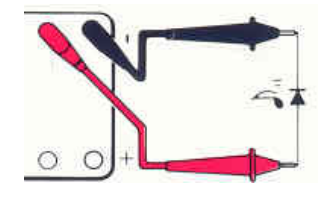
\includegraphics[width=2cm]{imagenes/sentido1.png}
\vspace{0.2cm}
} & & & & \\
\hline
\parbox[c][2.5cm][c]{2.5cm}{\centering % Espacio para imagen de sentido 2
\vspace{0.2cm}
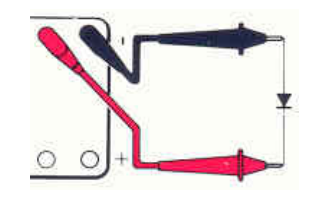
\includegraphics[width=2cm]{imagenes/sentido2.png}
\vspace{0.2cm}
} & & & & \\
\hline
\end{tabular}
\caption{Mediciones de diodos con multímetro}
\end{table}

(ADJUNTAR FOTOS DE MEDICIONES)

Como se puede observar en la tablra... (CONCLUSIONES)

